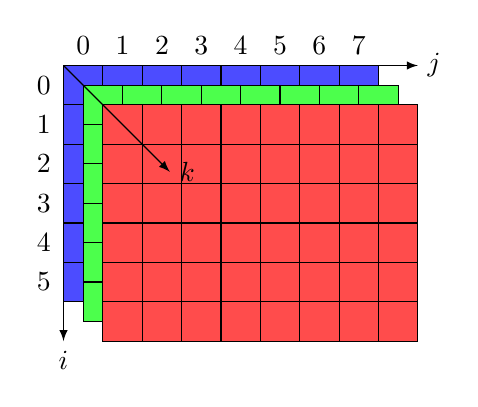
\begin{tikzpicture}[scale=0.5]
	\draw[fill=blue!70] (0,0) rectangle (8,6);
	\foreach \i in {0,1,...,6}
	{
		\draw (0,\i) -- ++(8,0);
	}
	\foreach \i in {0,1,...,5}
	{
		\node at (-0.5, 5.5 - \i) {$\i$};
	}	
	\foreach \j in {0,1,...,8}
	{
		\draw (\j,0) -- ++(0,6);
	}
	\foreach \j in {0,1,...,7}
	{
		\node at (\j + 0.5, 6.5) {$\j$};
	}		
	\draw[-latex] (0,6) -- ++(0,-7) node[anchor=north] {$i$};		
	\draw[-latex] (0,6) -- ++(9,0) node[anchor=west] {$j$};

\begin{scope}[xshift=0.5cm, yshift=-0.5cm]
	\draw[fill=green!70] (0,0) rectangle (8,6);
	\foreach \i in {0,1,...,6}
	{
		\draw (0,\i) -- ++(8,0);
	}

	\foreach \j in {0,1,...,8}
	{
		\draw (\j,0) -- ++(0,6);
	}

\end{scope}


\begin{scope}[xshift=1cm, yshift=-1cm]
	\draw[fill=red!70] (0,0) rectangle (8,6);
	\foreach \i in {0,1,...,6}
	{
		\draw (0,\i) -- ++(8,0);
	}

	\foreach \j in {0,1,...,8}
	{
		\draw (\j,0) -- ++(0,6);
	}

\end{scope}

\draw[-latex] (0,6) -- ++(2.7,-2.7) node[anchor=west] {$k$};
	
\end{tikzpicture} 